\documentclass[conference,a4paper]{IEEEtran}
% conference: differentiate between journals and conference format
% a4paper: set the paper size to A4
%% Support sites:
%% http://www.michaelshell.org/tex/ieeetran/
%% http://www.ctan.org/tex-archive/macros/latex/contrib/IEEEtran/
%% and
%% http://www.ieee.org/

%\IEEEoverridecommandlockouts
% The preceding line is only needed to identify funding in the first footnote. If that is unneeded, please comment it out.

%% Package inclusion
%% More details on what many of these packages do are at the end of this file
\usepackage[T1]{fontenc}%T1 fonts have Þ and ð
\usepackage[utf8]{inputenc}% allows UTF encoding, needed for Icelandic characters


\usepackage{cite}%reorganizing citation numbers
\usepackage[cmex10]{amsmath}%American Math Society(AMS) math formatting
\usepackage{amssymb,amsfonts}%AMS extra symbols and fonts
\interdisplaylinepenalty=2500%allow line breaks in multi-line formulas
\usepackage{array}%enhanced table tools
\usepackage[caption=false,font=footnotesize]{subfig}%sub-figures under a main figure
\usepackage{dblfloatfix}%fix double column figure ordering and placement

\usepackage{algorithmic}%writing algorithms
\usepackage{graphicx}%graphics inclusion
% declare the path(s) where your graphic files are
\graphicspath{{graphics/}{moregraphics/}}
% and their extensions so you won't have to specify these with
% every instance of \includegraphics
\DeclareGraphicsExtensions{.pdf,.PDF,.jpeg,.JPEG,.jpg,.JPEG,.png,.PNG}

\usepackage{booktabs}%pretty lines in tables: \toprule,\columnrule,\bottomrule

\usepackage{siunitx}%SI unit formatting:  \SI{9.8}{\meter\per\second} and \si{\meter\per\second\square}

\usepackage{textcomp}%special symbols not in all fonts
\usepackage{xcolor}%color macros
\usepackage[spaces,hyphens]{url}

% *** Do not adjust lengths that control margins, column widths, etc. ***
% *** Do not use packages that alter fonts (such as pslatex).         ***
% There should be no need to do such things with IEEEtran.cls V1.6 and later.
% (Unless specifically asked to do so by the journal or conference you plan
% to submit to, of course. )

% correct bad hyphenation here
\hyphenation{op-tical net-works semi-conduc-tor}

\def\BibTeX{{\rm B\kern-.05em{\sc i\kern-.025em b}\kern-.08em
    T\kern-.1667em\lower.7ex\hbox{E}\kern-.125emX}}

\begin{document}

\title{Team 00: My Project Title}

\author{\IEEEauthorblockN{Joseph Timothy Foley}
\IEEEauthorblockA{School of Science and Engineering\\
Reykjavík University\\
101 Reykjavík, Iceland\\
foley AT RU.IS}
\and
% We use a name with the special icelandic characters to make sure
% the fonts and encoding were setup properly.
\IEEEauthorblockN{2\textsuperscript{nd} Þórður Ægir Össurson}
\IEEEauthorblockA{\textit{dept. name of organization (of Aff.)} \\
\textit{name of organization (of Aff.)}\\
City, Country \\
email address}
\and
\IEEEauthorblockN{3\textsuperscript{rd} Given Name Surname}
\IEEEauthorblockA{\textit{dept. name of organization (of Aff.)} \\
\textit{name of organization (of Aff.)}\\
City, Country \\
email address}
\and
\IEEEauthorblockN{4\textsuperscript{th} Given Name Surname}
\IEEEauthorblockA{\textit{dept. name of organization (of Aff.)} \\
\textit{name of organization (of Aff.)}\\
City, Country \\
email address}
\and
\IEEEauthorblockN{5\textsuperscript{th} Given Name Surname}
\IEEEauthorblockA{\textit{dept. name of organization (of Aff.)} \\
\textit{name of organization (of Aff.)}\\
City, Country \\
email address}
\and
\IEEEauthorblockN{6\textsuperscript{th} Given Name Surname}
\IEEEauthorblockA{\textit{dept. name of organization (of Aff.)} \\
\textit{name of organization (of Aff.)}\\
City, Country \\
email address}
}

\maketitle
\begin{abstract}
  Beal recommends that you consolidate the whole paper into 5 sentences in 250 words or preferably less:
  \begin{enumerate}
  \item There is a problem with these real effects or this situation.
  \item Here is a general approach to fixing it.
  \item We now present this particular step.
  \item In particular, we did these very specific things.
  \item Success is confirmed by this quantitative result.
  \end{enumerate}

  Remember that an abstract often gets separated from the report:
  {\em do Not Use Symbols, Special Characters, Footnotes, or Math in Paper Title or Abstract!\/}

%This document is a model and instructions for \LaTeX.
%This and the IEEEtran.cls file define the components of your paper [title, text, heads, etc.]. *CRITICAL: Do Not Use Symbols, Special Characters, Footnotes, 
%or Math in Paper Title or Abstract.
\end{abstract}

\begin{IEEEkeywords}
component, formatting, style, styling, insert
\end{IEEEkeywords}

% You must have at least 2 lines in the paragraph with the drop letter
% (should never be an issue)
\section*{Instructions}
For LaTeX help, you should first consult Kopka and Daly's book~\cite{kopka1999guidetolatex}.
Before you start anything else, put your names in the top and add the team number in the title.
Sections that do not have numbers are provided for instructional use and should be removed before the paper is submitted.
You should start by picking if this will be an IMRAD or Design paper, then delete the other set of sections.
Before submitting, it is highly recommended to do a spell-check and a grammar check such as \url{http://grammarly.com}.
Pasting in the \LaTeX{} source code into Grammarly has worked well for the instructor.
We highly recommend using a reference manager like JabRef or Zotero to export a BibTeX file instead of managing the \path{references.bib} by hand.
You can easily remove the extra instructions in the appendix 

\section*{Academic Honesty}
If any part of your report is plagiarized (from another group, the internet, or anywhere else) or your references are not properly cited, you will receive a grade of zero on the entire assignment.
This is in compliance with Reykjavík University's Code of Ethics at \url{http://en.ru.is/the-university/ru-code-of-ethics/}\footnote{See Item 8 and General Rules on Study and Examinations}.
See also ``Study and Examination rules'' at \url{http://en.ru.is/studies/study--and-examination-rules/}\footnote{Article 4.5}
and ``Reglur um verkefnavinnu'' at \url{http://www.ru.is/namid/reglur/hugverk}.
For your reference, here is a link to guidelines defining plagiarism and discussing how to avoid it (from the
University of Oxford):

\url{https://www.ox.ac.uk/students/academic/guidance/skills/plagiarism?wssl=1}


\section*{IMRAD Paper}
This set of sections if for if you are following the IMRAD format.
Delete the ``Design Paper'' headings if you have chosen this format.

\section{Introduction}\label{sec:intro1}
Etablish context for the report.
Include background on the main scientific concept(s) and citations

State the objective(s) for the lab or concept.
Why did you perform the experiment?
Why did you investigate this issue
\subsection{Subsection Heading Here}\label{sec:subhead1}
Subsection text here.


\subsubsection{Subsubsection Heading Here}\label{sec:subsubhead1}
Subsubsection text here.


% An example of a floating figure using the graphicx package.
% Note that \label must occur AFTER (or within) \caption.
% For figures, \caption should occur after the \includegraphics.
% Note that IEEEtran v1.7 and later has special internal code that
% is designed to preserve the operation of \label within \caption
% even when the captionsoff option is in effect. However, because
% of issues like this, it may be the safest practice to put all your
% \label just after \caption rather than within \caption{}.
%
% Reminder: the "draftcls" or "draftclsnofoot", not "draft", class
% option should be used if it is desired that the figures are to be
% displayed while in draft mode.
%
%\begin{figure}[!t]
%\centering
%\includegraphics[width=2.5in]{myfigure}
% where an .eps filename suffix will be assumed under latex, 
% and a .pdf suffix will be assumed for pdflatex; or what has been declared
% via \DeclareGraphicsExtensions.
%\caption{Simulation Results.}
%\label{fig_sim}
%\end{figure}

% Note that IEEE typically puts floats only at the top, even when this
% results in a large percentage of a column being occupied by floats.


% An example of a double column floating figure using two subfigures.
% (The subfig.sty package must be loaded for this to work.)
% The subfigure \label commands are set within each subfloat command,
% and the \label for the overall figure must come after \caption.
% \hfil is used as a separator to get equal spacing.
% Watch out that the combined width of all the subfigures on a 
% line do not exceed the text width or a line break will occur.
%
%\begin{figure*}[!t]
%\centering
%\subfloat[Case I]{\includegraphics[width=2.5in]{box}%
%\label{fig_first_case}}
%\hfil
%\subfloat[Case II]{\includegraphics[width=2.5in]{box}%
%\label{fig_second_case}}
%\caption{Simulation results.}
%\label{fig_sim}
%\end{figure*}
%
% Note that often IEEE papers with subfigures do not employ subfigure
% captions (using the optional argument to \subfloat[]), but instead will
% reference/describe all of them (a), (b), etc., within the main caption.


% An example of a floating table. Note that, for IEEE style tables, the 
% \caption command should come BEFORE the table. Table text will default to
% \footnotesize as IEEE normally uses this smaller font for tables.
% The \label must come after \caption as always.
%
%\begin{table}[!t]
%% increase table row spacing, adjust to taste
%\renewcommand{\arraystretch}{1.3}
% if using array.sty, it might be a good idea to tweak the value of
% \extrarowheight as needed to properly center the text within the cells
%\caption{An Example of a Table}
%\label{table_example}
%\centering
%% Some packages, such as MDW tools, offer better commands for making tables
%% than the plain LaTeX2e tabular which is used here.
%\begin{tabular}{|c||c|}
%\hline
%One & Two\\
%\hline
%Three & Four\\
%\hline
%\end{tabular}
%\end{table}


% Note that IEEE does not put floats in the very first column - or typically
% anywhere on the first page for that matter. Also, in-text middle ("here")
% positioning is not used. Most IEEE journals/conferences use top floats
% exclusively. Note that, LaTeX2e, unlike IEEE journals/conferences, places
% footnotes above bottom floats. This can be corrected via the \fnbelowfloat
% command of the stfloats package.

\section{Methods and Materials}\label{sec:methodsnmaterials}
Describe how you performed the lab.
Note any deviations from what you were supposed to do.
Use full sentences (tell a narrative story).
Provide enough detail such that people with similar experience as you could repeat the experiment.

\section{Results}\label{sec:results}
Create tables, plots, or drawings (“visual aids”) to present your data.
Describe your visual aids in full sentences.

What was your testing strategy?  What kinds of tests were performed?
Be very specific.
How did your system perform?
Make sure that there is a table/list indicating your system's quantitative performance.
As a simple example, refer to Table~\ref{table:testing}

\begin{table}
\centering
\caption{Happy Fun Ball test results}\label{table:testing}
\begin{tabular}{lll}
  \toprule
  {\bf Feature} &{\bf Trials} &{\bf Explanation}\\
  \midrule
  Ball rolls down \SI{30}{\degree} slope &10/10 &\\
  Ball rolls up 10 stairs   &2/10 &Motor failed\\
  Ball stays inflated for 24 hours &10/10 &\\
  Ball floats in water for 24 hours &10/10 &\\
  \bottomrule
\end{tabular}
\end{table}

\begin{figure}
\centering
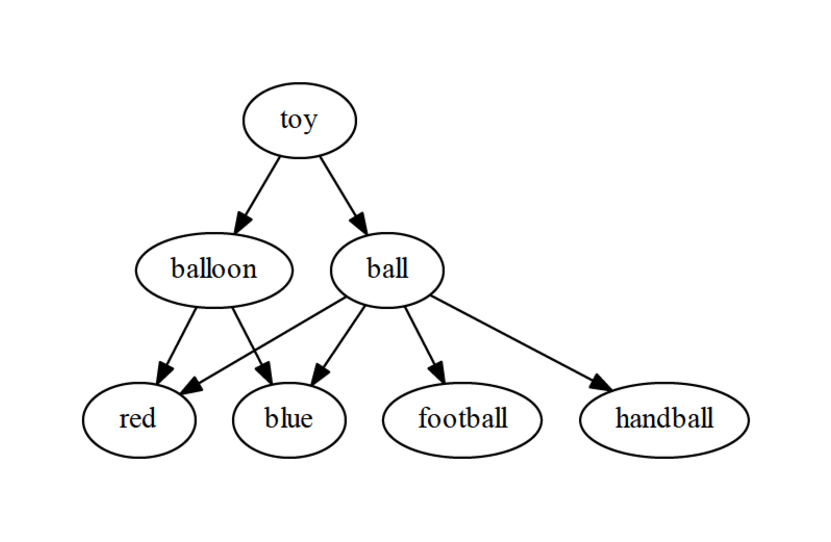
\includegraphics[width=\columnwidth,height=\textwidth,keepaspectratio]{mddgraph}
\caption{Modular Dependency Diagram of ``Toy'' object}\label{fig:mddgraph}
\end{figure}
\emph{NOTE: Figures and Tables need to be properly formatted and
  referenced in the text. Number figures/tables consecutively, include
  captions, and refer to the figures/tables in the text
  e.g. Figure~\ref{fig:mddgraph}. Equations need to be numbered consecutively as well.  Equations need to have each of their variables defined when they are first used or redefined.  If you need to refer to particular places in the document, use numbered references.  When you put a label{} command }

As an example of an equation, in Equation~\eqref{eq:freq} is the relationship between angular frequency and hertz:
\begin{equation}
f = \frac{1}{T} = \frac{1}{2\pi\omega}\label{eq:freq}
\end{equation}
where $f$ is frequency in \si{\hertz}, $T$ is period in \si{\second}, and
$\omega$ is angular frequency in \si{\radian\per\second}.



\section{Discussion}\label{sec:discussion}
Discuss what the results mean in the context of the concepts from the Introduction~(Section~\ref{sec:intro1}).
Offer explanation for any unanticipated results.


\section{Conclusion}\label{sec:conclusion1}
Summarize main conclusions (details!).
State if objectives were met.
Put forth ideas for follow-up experiments

\section*{Design Paper}
This set of sections is for if you are following the Design format.
Delete the ``IMRAD'' headings if you have chosen this format.

\section{Introduction}\label{sec:introduction2}
What is the problem and who cares about it\footnote{Effectively identifying the end-user and/or customer}?
What do they need in terms of a solution?
What needs are not being met?
What is the history of this technology or concept?

\section{Prior Art}\label{sec:priorart}
Search the internet and books to find out what people are currently doing in this area of research.
How is the problem currently addressed?  
Who and what is trying to solve it, especially the current state of the art?  

How do they compare to your general idea (preferably quantitatively)?
\begin{itemize}
\item E.g. You can’t say something is cheaper unless you have estimated costs
\item Avoid using the word “good” and “great”
\end{itemize}

\section{Design}\label{sec:design}
Build a list of requirements.
We suggest using Axiomatic Design developed by Nam P. Suh of MIT which uses Functional Requirements that start with a verb/action and are verifiable\cite{suh1990principles,suh1998adsystems,suh2005complexity}.

Then map these requirements to how they will be met.
Axiomatic Design does this with a list of Design Parameters starting with a noun/quantity that is measurable.
An example of this mapping can be found in Table~\ref{tab:first_level-frdp}

\begin{table}
  \center
  \caption{First level FR-DP mapping.~\cite{gerhard2016suretrack}}\label{tab:first_level-frdp}
  \begin{tabular}{lll} \toprule
    ID& Functional Requirement & Design Parameter \\ \midrule 
    1&Contain product&Main weldment\\
    2&Move product&Support system\\
    3&Discharge product &Discharge system\\
    \bottomrule
  \end{tabular}
\end{table}

Give more details on implementation.


\section{Analysis}\label{sec:analysis}
Use analytical tools (CAD, equations, simulations, or prototypes) to test if the design could plausibly solve the problems mentioned in the Introduction~(Section~\ref{sec:introduction2})
Put lots of graphics here!  
Put lots of Calculations and data!
Give an explanation of how to interpret them

\begin{figure}[htbp]
  \centering
  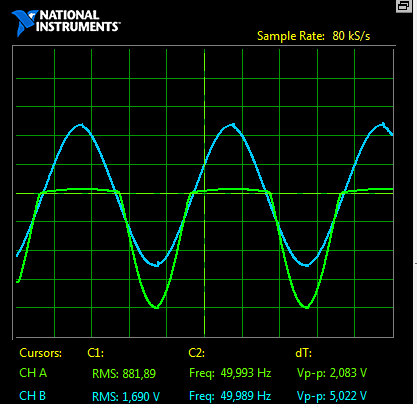
\includegraphics[width=\columnwidth,height=\textheight,keepaspectratio]{scope1}
  \caption{Oscilloscope capture of the amplifier signal being rectified.}
  \label{fig:scope1}
\end{figure}


\section{Conclusion}\label{sec:conclusion2}
What are the important things to remember?
Go through each goal/requirement stated and evaluate if they were met.
Summarize the result and justify the conclusion.
Does this result indicate if it is worth further investigation?





% use section* for acknowledgment
\section*{Acknowledgment}
The authors would like to thank Jacob Beal of Raytheon/BBN for providing the presentation ``Prototype to Paper in 6 Easy Steps'' to give guidance on how to write an abstract~\cite{beal2016prototype}.
The authors would also like to thank Markéta Foley for her presentation on writing reports for the RU course T-106-LIF in 2012.




%trigger a \newpage just before the given reference
% number - used to balance the columns on the last page
% adjust value as needed - may need to be readjusted if
% the document is modified later
%\IEEEtriggeratref{8}
% The "triggered" command can be changed if desired:
%\IEEEtriggercmd{\enlargethispage{-5in}}

% references section

% can use a bibliography generated by BibTeX as a .bbl file
% BibTeX documentation can be easily obtained at:
% http://www.ctan.org/tex-archive/biblio/bibtex/contrib/doc/
% The IEEEtran BibTeX style support page is at:
% http://www.michaelshell.org/tex/ieeetran/bibtex/
\bibliographystyle{IEEEtran}
% argument is your BibTeX string definitions and bibliography database(s)
% \bibliography{IEEEabrv,../bib/paper}
\bibliography{references}

\appendix
\section{Introduction}
Conference papers do not normally have an appendix.
We put one in this case to differentiate the text guidelines from the original IEEE Sustainability template's instructions

Helpful resources for writing can be found at
\begin{itemize}
\item The Science of Scientific Writing:  \url{https://www.americanscientist.org/blog/the-long-view/the-science-of-scientific-writing}
\item Viginia Tech Engineering Communication Center: \url{https://www.vtecc.eng.vt.edu/
}
\end{itemize}


This document is a model and instructions for \LaTeX.
Please observe the conference page limits. 

\section{Ease of Use}

\subsection{Maintaining the Integrity of the Specifications}

The IEEEtran class file is used to format your paper and style the text. All margins, 
column widths, line spaces, and text fonts are prescribed; please do not 
alter them. You may note peculiarities. For example, the head margin
measures proportionately more than is customary. This measurement 
and others are deliberate, using specifications that anticipate your paper 
as one part of the entire proceedings, and not as an independent document. 
Please do not revise any of the current designations.

\section{Prepare Your Paper Before Styling}
Before you begin to format your paper, first write and save the content as a 
separate text file. Complete all content and organizational editing before 
formatting. Please note sections \ref{AA}--\ref{SCM} below for more information on 
proofreading, spelling and grammar.

Keep your text and graphic files separate until after the text has been 
formatted and styled. Do not number text heads---{\LaTeX} will do that 
for you.

\subsection{Abbreviations and Acronyms}\label{AA}
Define abbreviations and acronyms the first time they are used in the text, 
even after they have been defined in the abstract. Abbreviations such as 
IEEE, SI, MKS, CGS, ac, dc, and rms do not have to be defined. Do not use 
abbreviations in the title or heads unless they are unavoidable.

\subsection{Units}
\begin{itemize}
\item Use either SI (MKS) or CGS as primary units. (SI units are encouraged.) English units may be used as secondary units (in parentheses). An exception would be the use of English units as identifiers in trade, such as ``3.5-inch disk drive''.
\item Avoid combining SI and CGS units, such as current in amperes and magnetic field in oersteds. This often leads to confusion because equations do not balance dimensionally. If you must use mixed units, clearly state the units for each quantity that you use in an equation.
\item Do not mix complete spellings and abbreviations of units: ``Wb/m\textsuperscript{2}'' or ``webers per square meter'', not ``webers/m\textsuperscript{2}''. Spell out units when they appear in text: ``. . . a few henries'', not ``. . . a few H''.
\item Use a zero before decimal points: ``0.25'', not ``.25''. Use ``cm\textsuperscript{3}'', not ``cc''.)
\end{itemize}

\subsection{Equations}
Number equations consecutively. To make your 
equations more compact, you may use the solidus (~/~), the exp function, or 
appropriate exponents. Italicize Roman symbols for quantities and variables, 
but not Greek symbols. Use a long dash rather than a hyphen for a minus 
sign. Punctuate equations with commas or periods when they are part of a 
sentence, as in:
\begin{equation}
a+b=\gamma\label{eq}
\end{equation}

Be sure that the 
symbols in your equation have been defined before or immediately following 
the equation. Use ``\eqref{eq}'', not ``Eq.~\eqref{eq}'' or ``equation \eqref{eq}'', except at 
the beginning of a sentence: ``Equation \eqref{eq} is . . .''

\subsection{\LaTeX-Specific Advice}

Please use ``soft'' (e.g., \verb|\eqref{Eq}|) cross references instead
of ``hard'' references (e.g., \verb|(1)|). That will make it possible
to combine sections, add equations, or change the order of figures or
citations without having to go through the file line by line.

Please don't use the \verb|{eqnarray}| equation environment. Use
\verb|{align}| or \verb|{IEEEeqnarray}| instead. The \verb|{eqnarray}|
environment leaves unsightly spaces around relation symbols.

Please note that the \verb|{subequations}| environment in {\LaTeX}
will increment the main equation counter even when there are no
equation numbers displayed. If you forget that, you might write an
article in which the equation numbers skip from (17) to (20), causing
the copy editors to wonder if you've discovered a new method of
counting.

{\BibTeX} does not work by magic. It doesn't get the bibliographic
data from thin air but from .bib files. If you use {\BibTeX} to produce a
bibliography you must send the .bib files. 

{\LaTeX} can't read your mind. If you assign the same label to a
subsubsection and a table, you might find that Table I has been cross
referenced as Table IV-B3. 

{\LaTeX} does not have precognitive abilities. If you put a
\verb|\label| command before the command that updates the counter it's
supposed to be using, the label will pick up the last counter to be
cross referenced instead. In particular, a \verb|\label| command
should not go before the caption of a figure or a table.

Do not use \verb|\nonumber| inside the \verb|{array}| environment. It
will not stop equation numbers inside \verb|{array}| (there won't be
any anyway) and it might stop a wanted equation number in the
surrounding equation.

\subsection{Some Common Mistakes}\label{SCM}
\begin{itemize}
\item The word ``data'' is plural, not singular.
\item The subscript for the permeability of vacuum $\mu_{0}$, and other common scientific constants, is zero with subscript formatting, not a lowercase letter ``o''.
\item In American English, commas, semicolons, periods, question and exclamation marks are located within quotation marks only when a complete thought or name is cited, such as a title or full quotation. When quotation marks are used, instead of a bold or italic typeface, to highlight a word or phrase, punctuation should appear outside of the quotation marks. A parenthetical phrase or statement at the end of a sentence is punctuated outside of the closing parenthesis (like this). (A parenthetical sentence is punctuated within the parentheses.)
\item A graph within a graph is an ``inset'', not an ``insert''. The word alternatively is preferred to the word ``alternately'' (unless you really mean something that alternates).
\item Do not use the word ``essentially'' to mean ``approximately'' or ``effectively''.
\item In your paper title, if the words ``that uses'' can accurately replace the word ``using'', capitalize the ``u''; if not, keep using lower-cased.
\item Be aware of the different meanings of the homophones ``affect'' and ``effect'', ``complement'' and ``compliment'', ``discreet'' and ``discrete'', ``principal'' and ``principle''.
\item Do not confuse ``imply'' and ``infer''.
\item The prefix ``non'' is not a word; it should be joined to the word it modifies, usually without a hyphen.
\item There is no period after the ``et'' in the Latin abbreviation ``et al.''.
\item The abbreviation ``i.e.'' means ``that is'', and the abbreviation ``e.g.'' means ``for example''.
\end{itemize}
An excellent style manual for science writers is \cite{b7}.

\subsection{Authors and Affiliations}
\textbf{The class file is designed for, but not limited to, six authors.} A 
minimum of one author is required for all conference articles. Author names 
should be listed starting from left to right and then moving down to the 
next line. This is the author sequence that will be used in future citations 
and by indexing services. Names should not be listed in columns nor group by 
affiliation. Please keep your affiliations as succinct as possible (for 
example, do not differentiate among departments of the same organization).

\subsection{Identify the Headings}
Headings, or heads, are organizational devices that guide the reader through 
your paper. There are two types: component heads and text heads.

Component heads identify the different components of your paper and are not 
topically subordinate to each other. Examples include Acknowledgments and 
References and, for these, the correct style to use is ``Heading 5''. Use 
``figure caption'' for your Figure captions, and ``table head'' for your 
table title. Run-in heads, such as ``Abstract'', will require you to apply a 
style (in this case, italic) in addition to the style provided by the drop 
down menu to differentiate the head from the text.

Text heads organize the topics on a relational, hierarchical basis. For 
example, the paper title is the primary text head because all subsequent 
material relates and elaborates on this one topic. If there are two or more 
sub-topics, the next level head (uppercase Roman numerals) should be used 
and, conversely, if there are not at least two sub-topics, then no subheads 
should be introduced.

\subsection{Figures and Tables}
\paragraph{Positioning Figures and Tables} Place figures and tables at the top and 
bottom of columns. Avoid placing them in the middle of columns. Large 
figures and tables may span across both columns. Figure captions should be 
below the figures; table heads should appear above the tables. Insert 
figures and tables after they are cited in the text. Use the abbreviation 
``Fig.~\ref{fig}'', even at the beginning of a sentence.

\begin{table}[htbp]
\caption{Table Type Styles}
\begin{center}
\begin{tabular}{|c|c|c|c|}
\hline
\textbf{Table}&\multicolumn{3}{|c|}{\textbf{Table Column Head}} \\
\cline{2-4} 
\textbf{Head} & \textbf{\textit{Table column subhead}}& \textbf{\textit{Subhead}}& \textbf{\textit{Subhead}} \\
\hline
copy& More table copy$^{\mathrm{a}}$& &  \\
\hline
\multicolumn{4}{l}{$^{\mathrm{a}}$Sample of a Table footnote.}
\end{tabular}
\label{tab1}
\end{center}
\end{table}

\begin{table}[htbp]
  \centering
  \caption{Example of a book-style table}\label{tab:book-style}
  \begin{tabular}{ll}
    \toprule
    X &Y\\
    \midrule
    1 &1\\
    2 &4\\
    3 &9\\
    \bottomrule
  \end{tabular}
\end{table}

\begin{figure}[htbp]
\centerline{
\includegraphics[width=0.75\columnwidth,height=0.75\textheight,keepaspectratio]{ru-logo}}
\caption{Example of a figure caption.  This is the RU logo.}
\label{fig}
\end{figure}

Figure Labels: Use 8 point Times New Roman for Figure labels. Use words 
rather than symbols or abbreviations when writing Figure axis labels to 
avoid confusing the reader. As an example, write the quantity 
``Magnetization'', or ``Magnetization, M'', not just ``M''. If including 
units in the label, present them within parentheses. Do not label axes only 
with units. In the example, write ``Magnetization (A/m)'' or ``Magnetization 
\{A[m(1)]\}'', not just ``A/m''. Do not label axes with a ratio of 
quantities and units. For example, write ``Temperature (K)'', not 
``Temperature/K''.

\section*{Acknowledgment}

The preferred spelling of the word ``acknowledgment'' in America is without 
an ``e'' after the ``g''. Avoid the stilted expression ``one of us (R. B. 
G.) thanks $\ldots$''. Instead, try ``R. B. G. thanks$\ldots$''. Put sponsor 
acknowledgments in the unnumbered footnote on the first page.

\section*{References}
A comprehensive guide to working with the IEEE citation style by Michael Shell can be found at the Comprehensive Tex Archive Network~\cite{shell2015ieeetranbst}.

Please number citations consecutively within brackets \cite{b1}. The 
sentence punctuation follows the bracket \cite{b2}. Refer simply to the reference 
number, as in \cite{b3}---do not use ``Ref. \cite{b3}'' or ``reference \cite{b3}'' except at 
the beginning of a sentence: ``Reference \cite{b3} was the first $\ldots$''

Number footnotes separately in superscripts. Place the actual footnote at 
the bottom of the column in which it was cited. Do not put footnotes in the 
abstract or reference list. Use letters for table footnotes.

Unless there are six authors or more give all authors' names; do not use 
``et al.''. Papers that have not been published, even if they have been 
submitted for publication, should be cited as ``unpublished'' \cite{b4}. Papers 
that have been accepted for publication should be cited as ``in press'' \cite{b5}. 
Capitalize only the first word in a paper title, except for proper nouns and 
element symbols.

For papers published in translation journals, please give the English 
citation first, followed by the original foreign-language citation \cite{b6}.

% \begin{thebibliography}{00}
% \bibitem{b1} G. Eason, B. Noble, and I. N. Sneddon, ``On certain integrals of Lipschitz-Hankel type involving products of Bessel functions,'' Phil. Trans. Roy. Soc. London, vol. A247, pp. 529--551, April 1955.
% \bibitem{b2} J. Clerk Maxwell, A Treatise on Electricity and Magnetism, 3rd ed., vol. 2. Oxford: Clarendon, 1892, pp.68--73.
% \bibitem{b3} I. S. Jacobs and C. P. Bean, ``Fine particles, thin films and exchange anisotropy,'' in Magnetism, vol. III, G. T. Rado and H. Suhl, Eds. New York: Academic, 1963, pp. 271--350.
% \bibitem{b4} K. Elissa, ``Title of paper if known,'' unpublished.
% \bibitem{b5} R. Nicole, ``Title of paper with only first word capitalized,'' J. Name Stand. Abbrev., in press.
% \bibitem{b6} Y. Yorozu, M. Hirano, K. Oka, and Y. Tagawa, ``Electron spectroscopy studies on magneto-optical media and plastic substrate interface,'' IEEE Transl. J. Magn. Japan, vol. 2, pp. 740--741, August 1987 [Digests 9th Annual Conf. Magnetics Japan, p. 301, 1982].
% \bibitem{b7} M. Young, The Technical Writer's Handbook. Mill Valley, CA: University Science, 1989.
% \end{thebibliography}
% \vspace{12pt}
% \color{red}

% can use a bibliography generated by BibTeX as a .bbl file
% BibTeX documentation can be easily obtained at:
% http://www.ctan.org/tex-archive/biblio/bibtex/contrib/doc/
% The IEEEtran BibTeX style support page is at:
% http://www.michaelshell.org/tex/ieeetran/bibtex/
%\bibliographystyle{IEEEtran}
% argument is your BibTeX string definitions and bibliography database(s)
% \bibliography{IEEEabrv,../bib/paper}
%\bibliography{references}


IEEE conference templates contain guidance text for composing and formatting conference papers. Please ensure that all template text is removed from your conference paper prior to submission to the conference. Failure to remove the template text from your paper may result in your paper not being published.

\end{document}
%%% Description for the packages used at the beginning of this file


%\usepackage{cite}
% cite.sty was written by Donald Arseneau
% V1.6 and later of IEEEtran pre-defines the format of the cite.sty package
% \cite{} output to follow that of IEEE. Loading the cite package will
% result in citation numbers being automatically sorted and properly
% "compressed/ranged". e.g., [1], [9], [2], [7], [5], [6] without using
% cite.sty will become [1], [2], [5]--[7], [9] using cite.sty. cite.sty's
% \cite will automatically add leading space, if needed. Use cite.sty's
% noadjust option (cite.sty V3.8 and later) if you want to turn this off
% such as if a citation ever needs to be enclosed in parenthesis.
% cite.sty is already installed on most LaTeX systems. Be sure and use
% version 4.0 (2003-05-27) and later if using hyperref.sty. cite.sty does
% not currently provide for hyperlinked citations.
% The latest version can be obtained at:
% http://www.ctan.org/tex-archive/macros/latex/contrib/cite/
% The documentation is contained in the cite.sty file itself.





%% Setup graphics inclusion
%\usepackage{graphicx}
% declare the path(s) where your graphic files are
%\graphicspath{{../pdf/}{../jpeg/}}
% and their extensions so you won't have to specify these with
% every instance of \includegraphics
%\DeclareGraphicsExtensions{.pdf,.PDF,.jpeg,.JPEG,.jpg,.JPEG,.png,.PNG}

% graphicx was written by David Carlisle and Sebastian Rahtz. It is
% required if you want graphics, photos, etc. graphicx.sty is already
% installed on most LaTeX systems. The latest version and documentation
% can be obtained at: 
% http://www.ctan.org/tex-archive/macros/latex/required/graphics/
% Another good source of documentation is "Using Imported Graphics in
% LaTeX2e" by Keith Reckdahl which can be found at:
% http://www.ctan.org/tex-archive/info/epslatex/
%
% latex, and pdflatex in dvi mode, support graphics in encapsulated
% postscript (.eps) format. pdflatex in pdf mode supports graphics
% in .pdf, .jpeg, .png and .mps (metapost) formats. Users should ensure
% that all non-photo figures use a vector format (.eps, .pdf, .mps) and
% not a bitmapped formats (.jpeg, .png). IEEE frowns on bitmapped formats
% which can result in "jaggedy"/blurry rendering of lines and letters as
% well as large increases in file sizes.
%
% You can find documentation about the pdfTeX application at:
% http://www.tug.org/applications/pdftex

% *** MATH PACKAGES ***
%
%\usepackage[cmex10]{amsmath}
% A popular package from the American Mathematical Society that provides
% many useful and powerful commands for dealing with mathematics. If using
% it, be sure to load this package with the cmex10 option to ensure that
% only type 1 fonts will utilized at all point sizes. Without this option,
% it is possible that some math symbols, particularly those within
% footnotes, will be rendered in bitmap form which will result in a
% document that can not be IEEE Xplore compliant!
%
% Also, note that the amsmath package sets \interdisplaylinepenalty to 10000
% thus preventing page breaks from occurring within multiline equations. Use:
%\interdisplaylinepenalty=2500
% after loading amsmath to restore such page breaks as IEEEtran.cls normally
% does. amsmath.sty is already installed on most LaTeX systems. The latest
% version and documentation can be obtained at:
% http://www.ctan.org/tex-archive/macros/latex/required/amslatex/math/


% *** ALIGNMENT PACKAGES ***
%
%\usepackage{array}
% Frank Mittelbach's and David Carlisle's array.sty patches and improves
% the standard LaTeX2e array and tabular environments to provide better
% appearance and additional user controls. As the default LaTeX2e table
% generation code is lacking to the point of almost being broken with
% respect to the quality of the end results, all users are strongly
% advised to use an enhanced (at the very least that provided by array.sty)
% set of table tools. array.sty is already installed on most systems. The
% latest version and documentation can be obtained at:
% http://www.ctan.org/tex-archive/macros/latex/required/tools/


% IEEEtran contains the IEEEeqnarray family of commands that can be used to
% generate multiline equations as well as matrices, tables, etc., of high
% quality.




% *** SUBFIGURE PACKAGES ***
%\usepackage[caption=false,font=footnotesize]{subfig}
% subfig.sty, written by Steven Douglas Cochran, is the modern replacement
% for subfigure.sty, the latter of which is no longer maintained and is
% incompatible with some LaTeX packages including fixltx2e. However,
% subfig.sty requires and automatically loads Axel Sommerfeldt's caption.sty
% which will override IEEEtran.cls' handling of captions and this will result
% in non-IEEE style figure/table captions. To prevent this problem, be sure
% and invoke subfig.sty's "caption=false" package option (available since
% subfig.sty version 1.3, 2005/06/28) as this is will preserve IEEEtran.cls
% handling of captions.
% Note that the Computer Society format requires a larger sans serif font
% than the serif footnote size font used in traditional IEEE formatting
% and thus the need to invoke different subfig.sty package options depending
% on whether compsoc mode has been enabled.
%
% The latest version and documentation of subfig.sty can be obtained at:
% http://www.ctan.org/tex-archive/macros/latex/contrib/subfig/




% *** FLOAT PACKAGES ***
%
%\usepackage{fixltx2e}
% fixltx2e, the successor to the earlier fix2col.sty, was written by
% Frank Mittelbach and David Carlisle. This package corrects a few problems
% in the LaTeX2e kernel, the most notable of which is that in current
% LaTeX2e releases, the ordering of single and double column floats is not
% guaranteed to be preserved. Thus, an unpatched LaTeX2e can allow a
% single column figure to be placed prior to an earlier double column
% figure. The latest version and documentation can be found at:
% http://www.ctan.org/tex-archive/macros/latex/base/


%\usepackage{stfloats}
% stfloats.sty was written by Sigitas Tolusis. This package gives LaTeX2e
% the ability to do double column floats at the bottom of the page as well
% as the top. (e.g., "\begin{figure*}[!b]" is not normally possible in
% LaTeX2e). It also provides a command:
%\fnbelowfloat
% to enable the placement of footnotes below bottom floats (the standard
% LaTeX2e kernel puts them above bottom floats). This is an invasive package
% which rewrites many portions of the LaTeX2e float routines. It may not work
% with other packages that modify the LaTeX2e float routines. The latest
% version and documentation can be obtained at:
% http://www.ctan.org/tex-archive/macros/latex/contrib/sttools/
% Do not use the stfloats baselinefloat ability as IEEE does not allow
% \baselineskip to stretch. Authors submitting work to the IEEE should note
% that IEEE rarely uses double column equations and that authors should try
% to avoid such use. Do not be tempted to use the cuted.sty or midfloat.sty
% packages (also by Sigitas Tolusis) as IEEE does not format its papers in
% such ways.
% Do not attempt to use stfloats with fixltx2e as they are incompatible.
% Instead, use Morten Hogholm'a dblfloatfix which combines the features
% of both fixltx2e and stfloats:
%
%\usepackage{dblfloatfix}
% The latest version can be found at:
% http://www.ctan.org/tex-archive/macros/latex/contrib/dblfloatfix/




% *** PDF, URL AND HYPERLINK PACKAGES ***
%
%\usepackage[spaces,hyphens]{url}
% url.sty was written by Donald Arseneau. It provides better support for
% handling and breaking URLs. url.sty is already installed on most LaTeX
% systems. The latest version and documentation can be obtained at:
% http://www.ctan.org/tex-archive/macros/latex/contrib/url/
% Basically, \url{my_url_here}.
%% options:
%%   spaces - allow breaks in URLs at spaces
%%   hyphens - allow breaks in URLS at hyphens
 

% *** Do not adjust lengths that control margins, column widths, etc. ***
% *** Do not use packages that alter fonts (such as pslatex).         ***
% There should be no need to do such things with IEEEtran.cls V1.6 and later.
% (Unless specifically asked to do so by the journal or conference you plan
% to submit to, of course. )


%%%%%%%%%%%%%%%%%%%% TeXStudio Magic Comments %%%%%%%%%%%%%%%%%%%%%
%% These comments that start with "!TeX" modify the way TeXStudio works
%% For details see http://texstudio.sourceforge.net/manual/current/usermanual_en.html   Section 4.10
%%
%% What encoding is the file in?
% !TeX encoding = UTF-8
%% What language should it be spellchecked?
% !TeX spellcheck = en_US
%% What program should I compile this document with?
% !TeX program = pdflatex
%% Which program should be used for generating the bibliography?
% !TeX TXS-program:bibliography = txs:///bibtex
%% This also sets the bibliography program for TeXShop and TeXWorks
% !BIB program = bibtex

%%%%%%%%%%%%%%%%%% Emacs Variables %%%%%%%%%%%%%%%%%%%%%%%
%%% These variables affect how the emacs editor works with the file
%%% Local Variables:
%%% mode: latex
%%% TeX-master: t
%%% End:
